\documentclass[english,xcolor=svgnames]{beamer}

\input{../../../../Templates/Latex/teachingslidesbeamer.tex}


% ===========================================================
% ===========================================================
% ===========================================================
\begin{document}

\title{Evidence on Nominal Rigidities}
\vspace{1cm}
\author[shortname]{
\begin{tabular}{c}
	Johannes Wieland \\ 
	\footnotesize \href{mailto:jfwieland@ucsd.edu}{jfwieland@ucsd.edu}  \\ 
\end{tabular}
}

\date{Spring \the\year}

\setbeamertemplate{footline}{}
\makebeamertitle
\setbeamertemplate{footline}[frame number]{}

\addtocounter{framenumber}{-1}

%%%%%%%%%%%%%%%%%%%%%%%%%%%%%%%%%%%%%%%%%%%%%%%%%%
\AtBeginSection[]{
\setbeamertemplate{footline}{}
  \frame<beamer>{ 

    \frametitle{Outline}   

    \tableofcontents[currentsection] 
  }
\setbeamertemplate{footline}[frame number]{}
\addtocounter{framenumber}{-1}
}

\AtBeginSubsection[]{
\setbeamertemplate{footline}{}
  \frame<beamer>{ 

    \frametitle{Outline}   

    \tableofcontents[currentsection,currentsubsection] 
  }
  \setbeamertemplate{footline}[frame number]{}
  \addtocounter{framenumber}{-1}
}

%%%%%%%%%%%%%%%%%%%%%%%%%%%%%%%%%%%%%%%%%%%%%%%%%%
\section{Intro}
%%%%%%%%%%%%%%%%%%%%%%%%%%%%%%%%%%%%%%%%%%%%%%%%%%

\begin{frame}
\frametitle{Empirical Evidence on Role of Money}
\begin{itemize}
	\item In the last class we reviewed the evidence for monetary (non-)neutrality from VARs.
	\item Today we will cover shortcomings of this approach.
	\item We will also look at other approaches to estimate the real effects of money.
\end{itemize}
\end{frame}


%%%%%%%%%%%%%%%%%%%%%%%%%%%%%%%%%%%%%%%%%%%%%%%%%%
\section{VAR Criticism}
%%%%%%%%%%%%%%%%%%%%%%%%%%%%%%%%%%%%%%%%%%%%%%%%%%


\begin{frame}
\frametitle{SVAR Criticisms
}
\begin{itemize}
	\item SVAR approach often described as imposing ``minimal identifying assumptions.''
	\begin{itemize}
		\item Make one innocuous timing assumption and, vo\`{i}la, you can identify the real effects of monetary policy.
		\item But timing assumption only rules out reverse causality.
	\end{itemize}
	\item Arguably bigger issue is an omitted variable bias:
	\begin{itemize}
		\item Suppose the central bank responds to a piece of information that the SVAR does not capture. E.g., the stock market tanks in anticipation of a recession.
		\item The SVAR interprets this as a monetary shock because it is a residual in the statistical model of the interest rate.
		\item The implied IRF for the monetary shock will be biased because it reflects the shock that causing this anticipation.
	\end{itemize} 
	\item[$\Rightarrow$] Require that the SVAR variables and lags account for the information the central bank uses to make its interest rate decisions.
	\item This is unlikely given forward-looking and episode-specific nature of central bank decisions.
\end{itemize}
\end{frame}

\begin{frame}
\frametitle{Example of likely OVB Bias
}
\centering
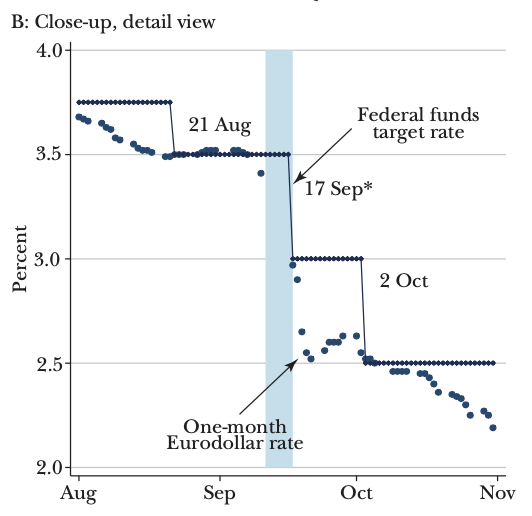
\includegraphics[scale=0.8]{../../Images/NS2018911.png}
\end{frame}


\begin{frame}
\frametitle{Further Criticisms of VARs
}
\begin{itemize}
	\item Symptom: ``Price puzzle''
	\begin{itemize}
		\item In many estimated VARs inflation rises with negative monetary shock.
		\begin{itemize}
			\item One answer is Fed is forward looking and rises rates when it (correctly) anticipated inflation.
			\item VAR omits variables that predict this inflation.
			\item Many VARs include an index of commodity prices to solve this problem.
		\end{itemize}
	\end{itemize}
	\item Other practical issues with VARs:
	\begin{itemize}
		\item Timing assumptions do not reflect real-time data availability, causing similar misspecification.
		\item Parameter instability.
	\end{itemize}
\end{itemize}
\end{frame}


%%%%%%%%%%%%%%%%%%%%%%%%%%%%%%%%%%%%%%%%%%%%%%%%%%
\section{Other Approaches}
%%%%%%%%%%%%%%%%%%%%%%%%%%%%%%%%%%%%%%%%%%%%%%%%%%

\begin{frame}
\frametitle{Other Approaches}
\begin{itemize}
	\item We may not like recursive VAR approach to identifying monetary shocks.
	\item Four other approaches that try to deal with causality more directly of which I want you to be aware.
\end{itemize}
\begin{enumerate}[1.]
	\item Large Shocks/Natural Experiments.
	\item Discontinuity-Based Approach.
	\item Narrative Approach.
	\item Controlling for Confounding Factors (includes VAR).
\end{enumerate}
\begin{itemize}
	\item Good summary: Section 4 of Nakamura and Steinsson (2018) ``Identification in Macroeconomics.''
\end{itemize}
\end{frame}

%%%%%%%%%%%%%%%%%%%%%%%%%%%%%%%%%%%%%%%%%%%%%%%%%%
\subsection{Large Shocks / Natural Experiments}
%%%%%%%%%%%%%%%%%%%%%%%%%%%%%%%%%%%%%%%%%%%%%%%%%%

\begin{frame}
\frametitle{Large Shocks / Natural Experiments}
\begin{itemize}
	\item Ideal evidence: Experiment where randomly change money supply in some places.
	\item Problem: Central banks are run by economists.
	\begin{itemize}
		\item Changes in money supply are not random!
	\end{itemize}
	\item Solution: Large shocks/Natural experiments. Examples:
	\begin{itemize}
		\item Hyperinflations: inflation tracks money supply.
		\item U.S. Great Depression (Friedman and Schwartz, 1963).
		\item Gold Standard and Great Depression (Eichengreen and Sachs,
1985; Hausman, Rhode, and Wieland, 2019).
%		\item Breakdown of Bretton Woods (Mussa, 1986).
		\item Volcker disinflation in early 1980s.
	\end{itemize}
	\item Idea: shock large relative to confounding factors.
\end{itemize}
\end{frame}

\begin{frame}
\frametitle{Large Shocks: Friedman and Schwartz (1963)}
\begin{itemize}
	\item Friedman and Schwartz (1963) famously argue that Fed made Great Depression worse.
	\item Focus on policy actions that are ``of major magnitude,'' not caused by other developments, sharp results that they compare to science experiment.
%	\begin{itemize}
%		\item But others have questioned since.
%	\end{itemize}
\end{itemize}
\centering
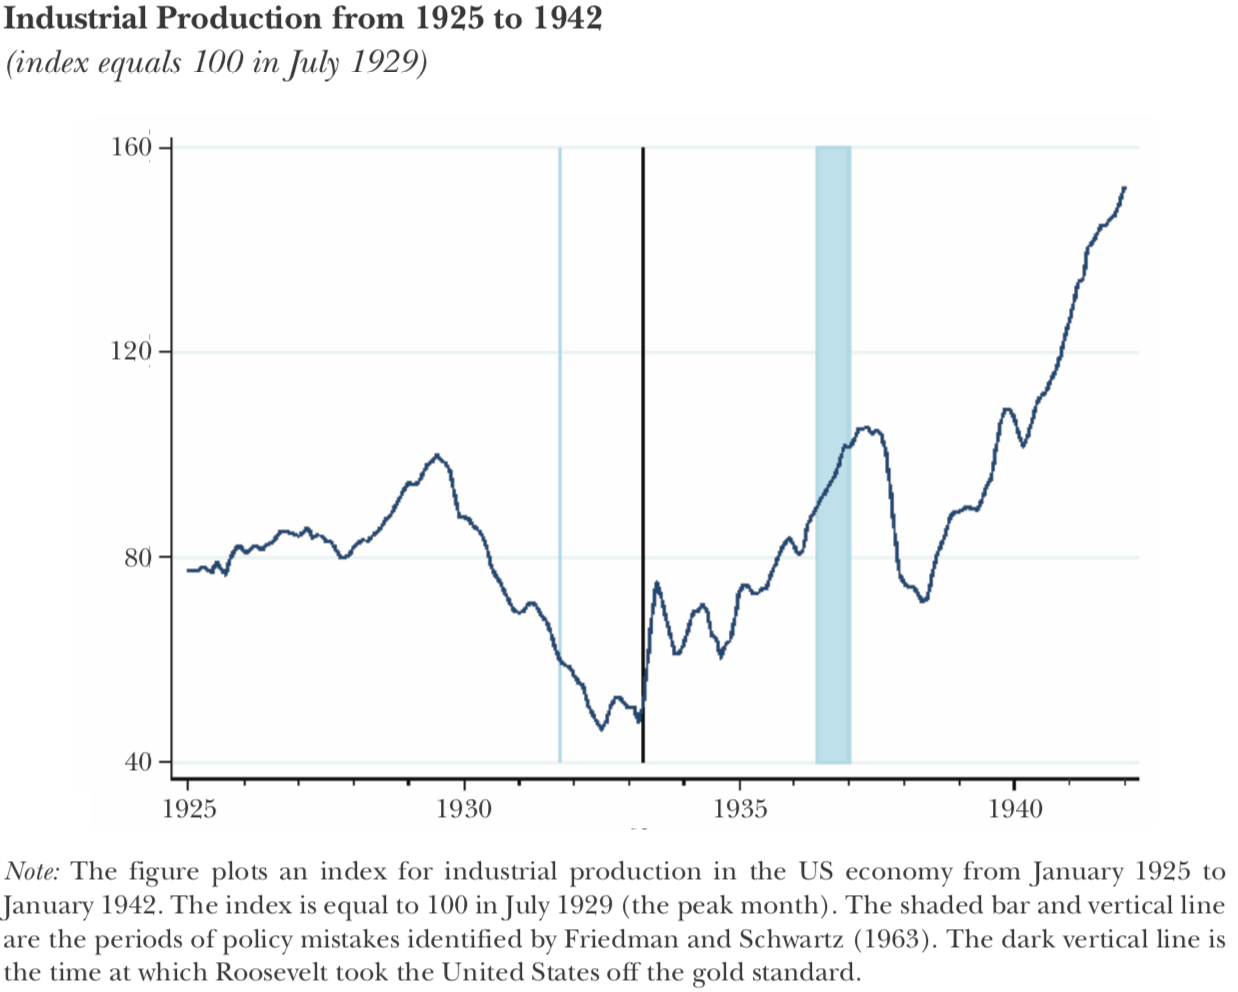
\includegraphics[scale=0.4]{../../Images/NS2018fs.png}	

\end{frame}


\begin{frame}
\frametitle{Volcker Disinflation}
\begin{itemize}
	\item In August 1979, Paul Volcker became chairman of the Federal Reserve. 
	\item First raised interest rates in October 1979, then backed off, then raised rapidly again in November 1980.
\end{itemize}
\centering
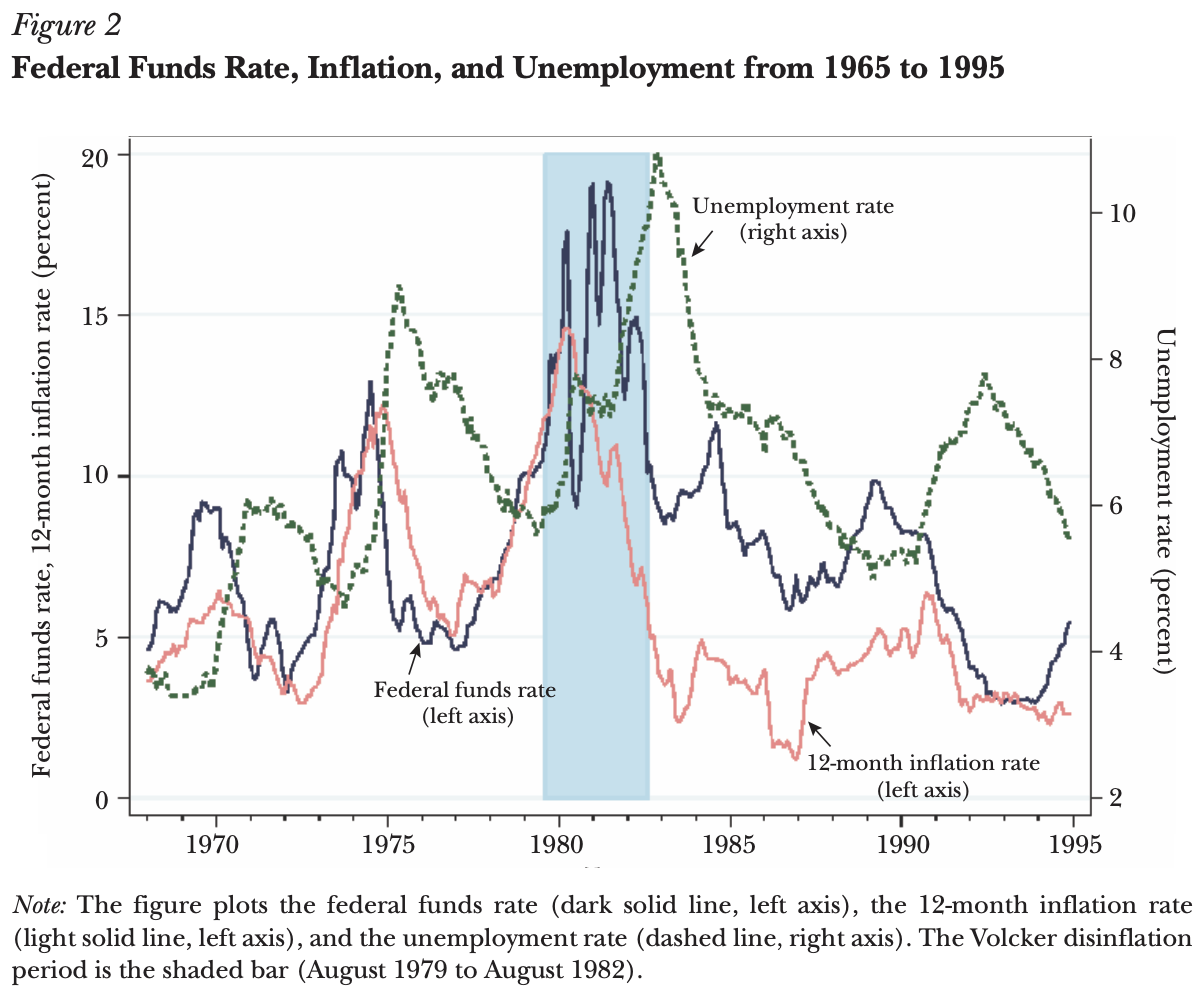
\includegraphics[scale=0.4]{../../Images/NS2018volcker.png}	

\end{frame}


\begin{frame}
\frametitle{France in 1724: A Surprise 45\% Deflation}
\begin{itemize}
	\item Money: coins with no face value.
	\begin{itemize}
		\item Government sets nominal value by decree, can change it
overnight and without warning.
	\end{itemize}
	\item Velde (2009) examines an episode where three times in 1724, French cut value of currency overnight by a cumulative 45\%.
	\begin{itemize}
		\item Ex: September 22, 1724 at 8am, all (formerly) 5 livre coins are now 4 livre coins.
		\item Why? King and his misters wanted to (before economists!).
		\item Revalue some in 1726.
	\end{itemize}
	\item Expectations:
	\begin{itemize}
		\item Had done before, but always fast inflations and gradual deflations.
		\item Velde argues these three deflations were ``unforetold.'' Kept secret to reduce capital losses by state.
	\end{itemize}
\end{itemize}
\end{frame}


\begin{frame}
\frametitle{Value of a Coin}
\centering
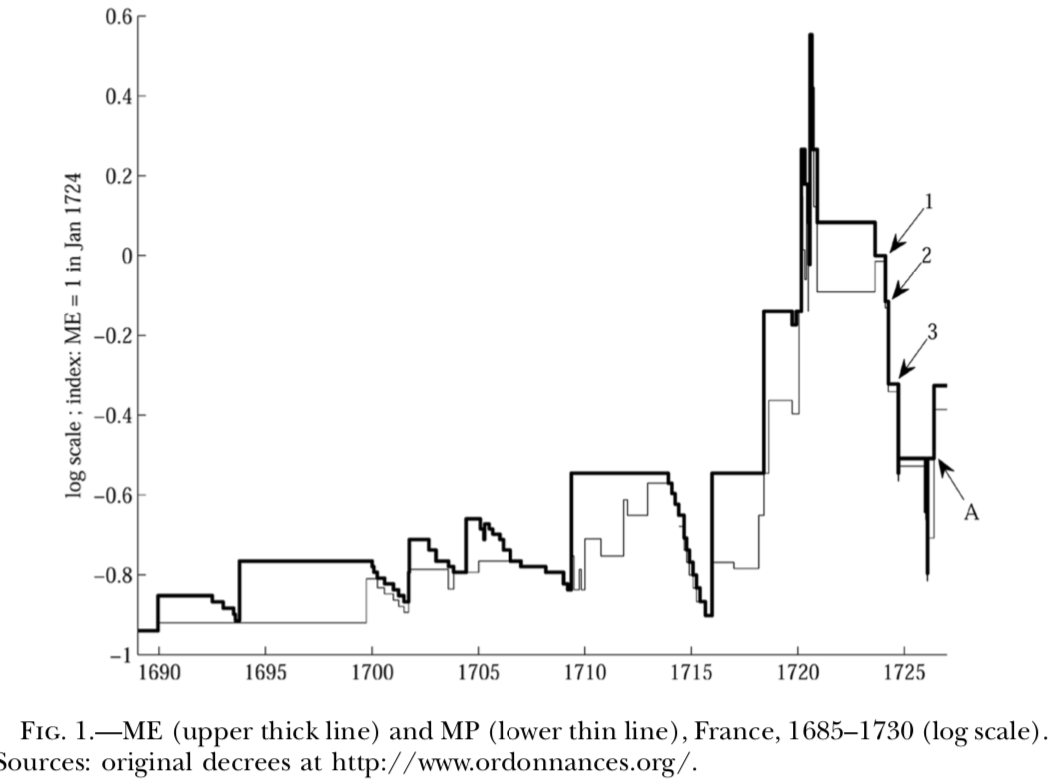
\includegraphics[scale=0.5]{../../Images/Velde2009coin.png}	
\end{frame}

\begin{frame}
\frametitle{Foreign Exchange Prices Adjust Instantaneously}
\centering
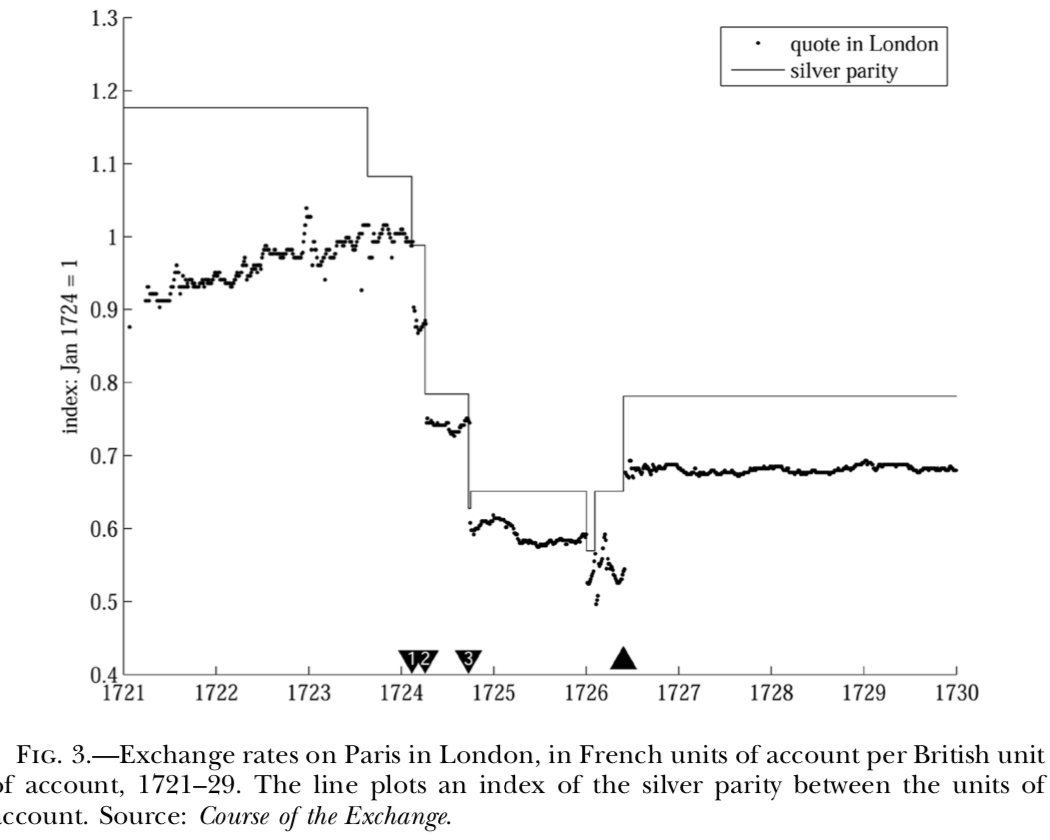
\includegraphics[scale=0.5]{../../Images/Velde2009fx.png}	
\end{frame}

\begin{frame}
\frametitle{Commodities and Goods Prices Fall Slowly}
\centering
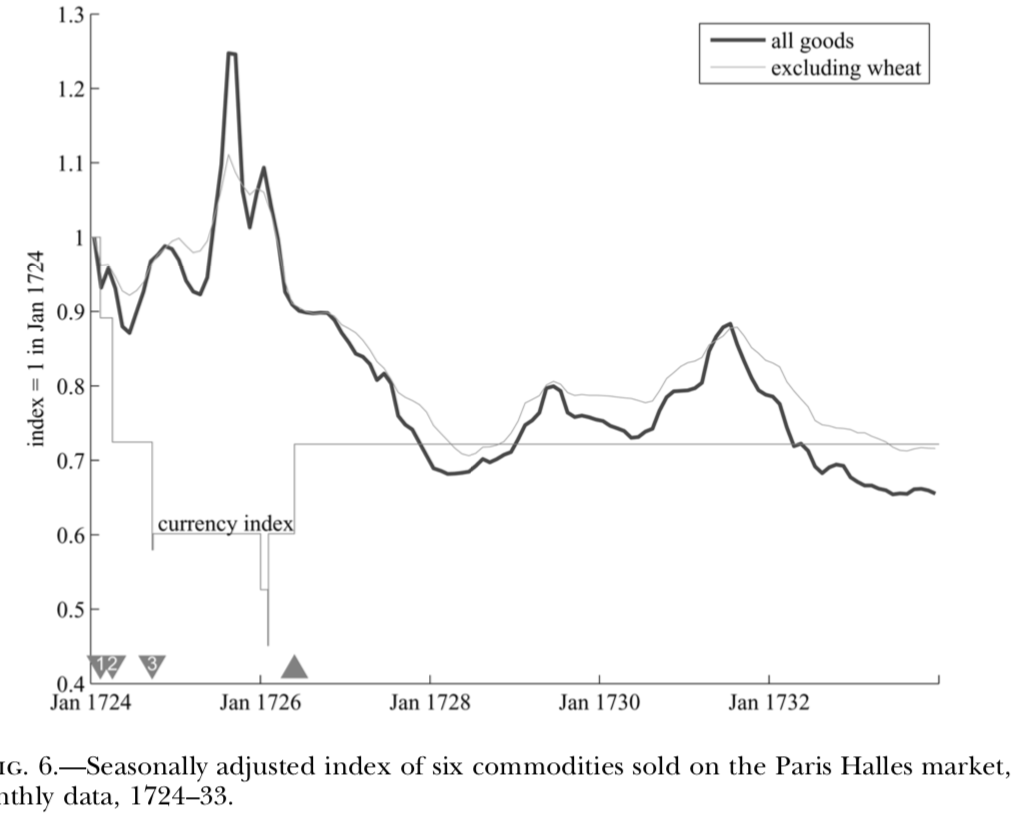
\includegraphics[scale=0.5]{../../Images/Velde2009commodities.png}	
\end{frame}

\begin{frame}
\frametitle{Industrial Sector Contracts 30\%}
\centering
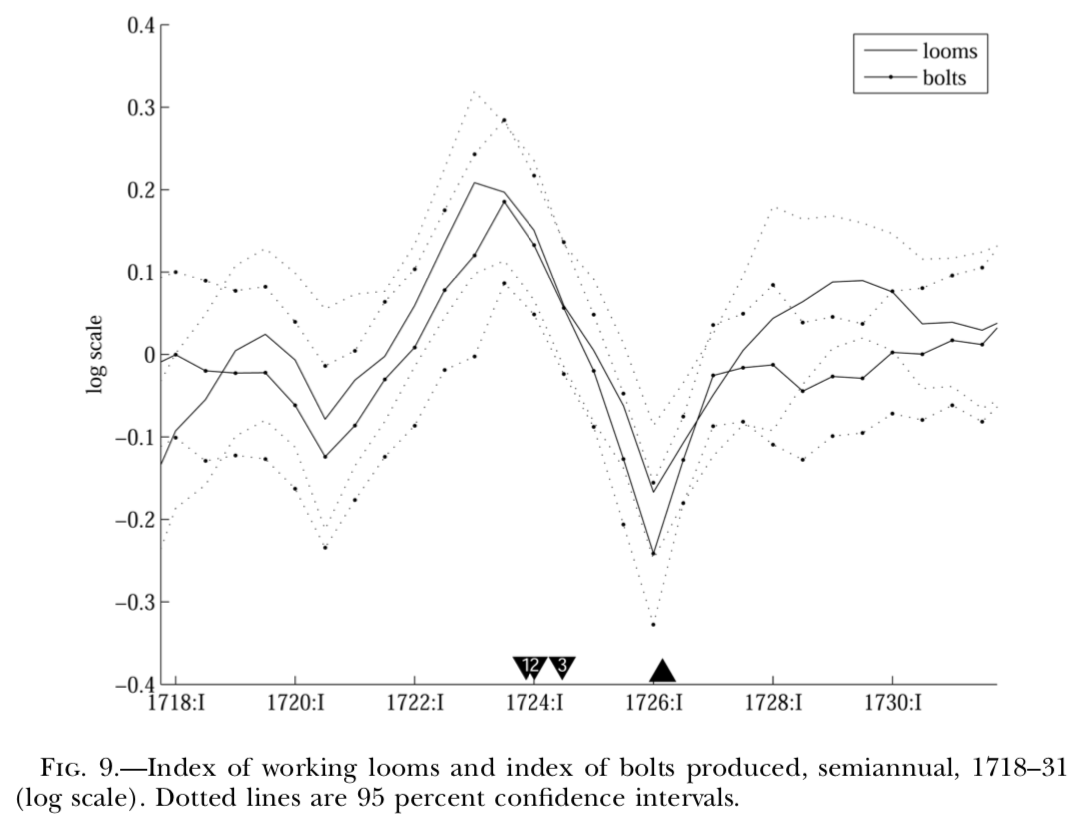
\includegraphics[scale=0.5]{../../Images/Velde2009textiles.png}	
\end{frame}

\begin{frame}
\frametitle[alignment=center]{Hausman, Rhode, Wieland (2019)}
\begin{itemize}
	\item Spring 1933: U.S. Abandons Gold
\end{itemize}
\centering
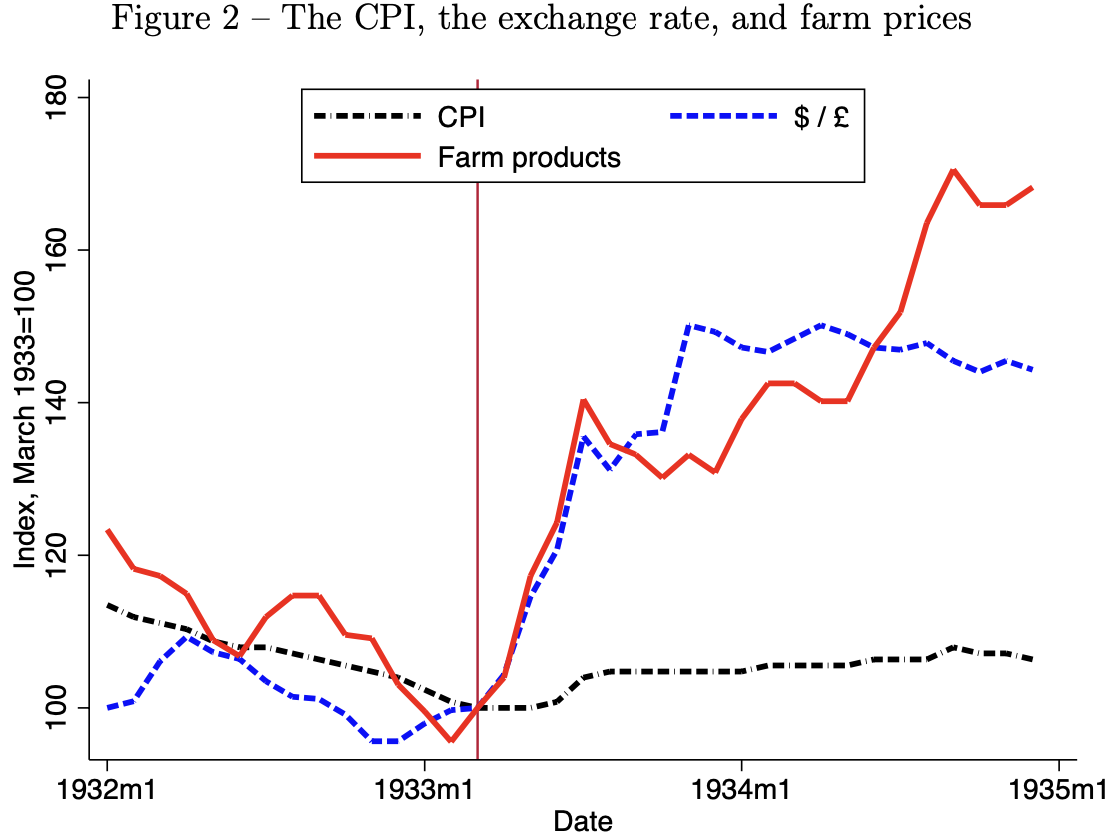
\includegraphics[scale=0.5]{../../Images/HRWFIG2.png}
\end{frame}

\begin{frame}
\frametitle[alignment=center]{Tradable Prices Rose}
\begin{itemize}
	\item Producers of tradables benefit. Almost exclusively farmers.
\end{itemize}
\centering
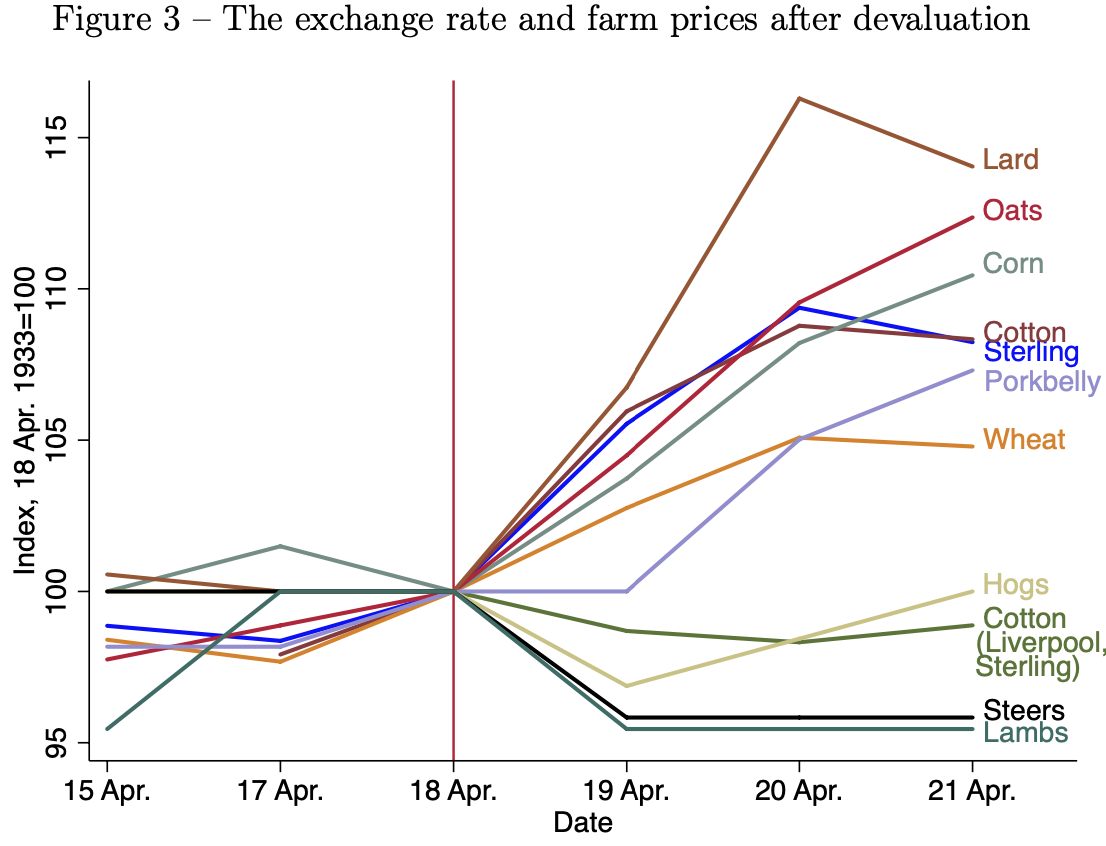
\includegraphics[scale=0.5]{../../Images/HRWFIG3.png}
\end{frame}

\begin{frame}
\frametitle[alignment=center]{Farm States Grow Faster}
\begin{itemize}
	\item Farm areas recover faster, especially those producing tradable goods.
\end{itemize}
\centering
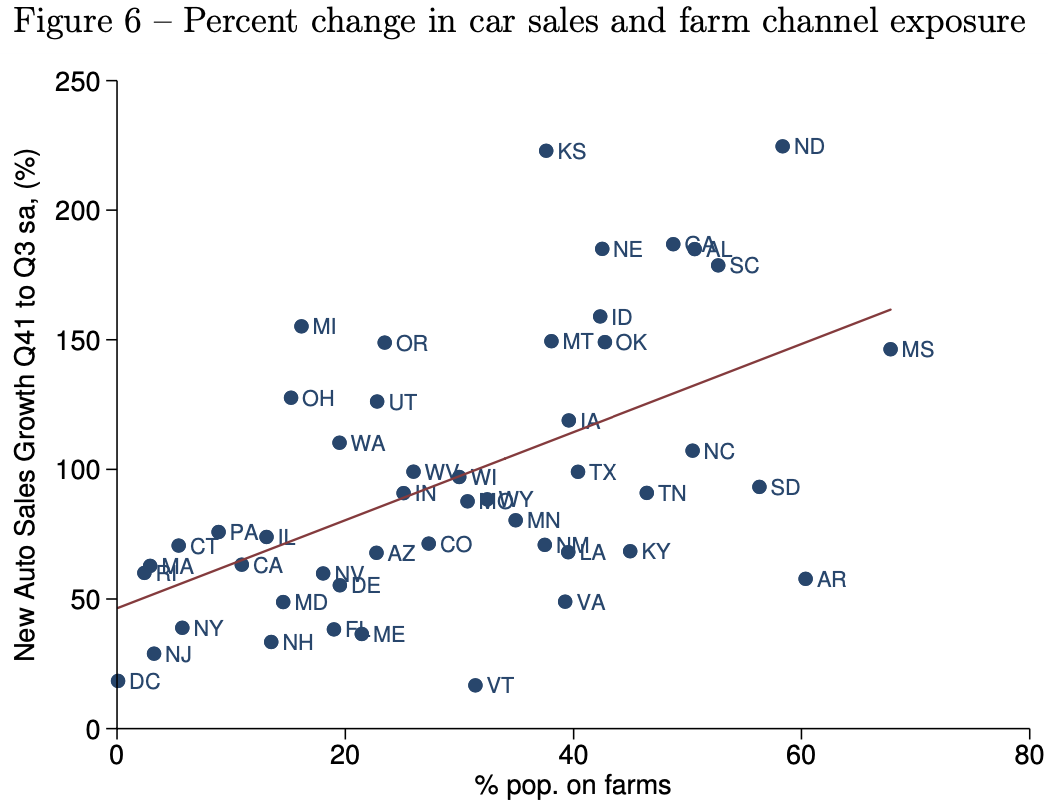
\includegraphics[scale=0.5]{../../Images/HRWFIG6a.png}
\end{frame}


%%%%%%%%%%%%%%%%%%%%%%%%%%%%%%%%%%%%%%%%%%%%%%%%%
\subsection{Discontinuity / High-Frequency}
%%%%%%%%%%%%%%%%%%%%%%%%%%%%%%%%%%%%%%%%%%%%%%%%%

\begin{frame}
\frametitle{Breakdown of Bretton Woods: Mussa (1986)}
\begin{itemize}
	\item In February 1973 Bretton Woods fixed exchange rate system breaks down.
	\begin{itemize}
		\item Discontinuous and purely monetary change.
		\item If monetary policy has no such effects, should not affect real
variables like real exchange rates.
	\end{itemize}
%	\item Monthly change in real Mark-Dollar exchange rate:
\end{itemize}
\centering
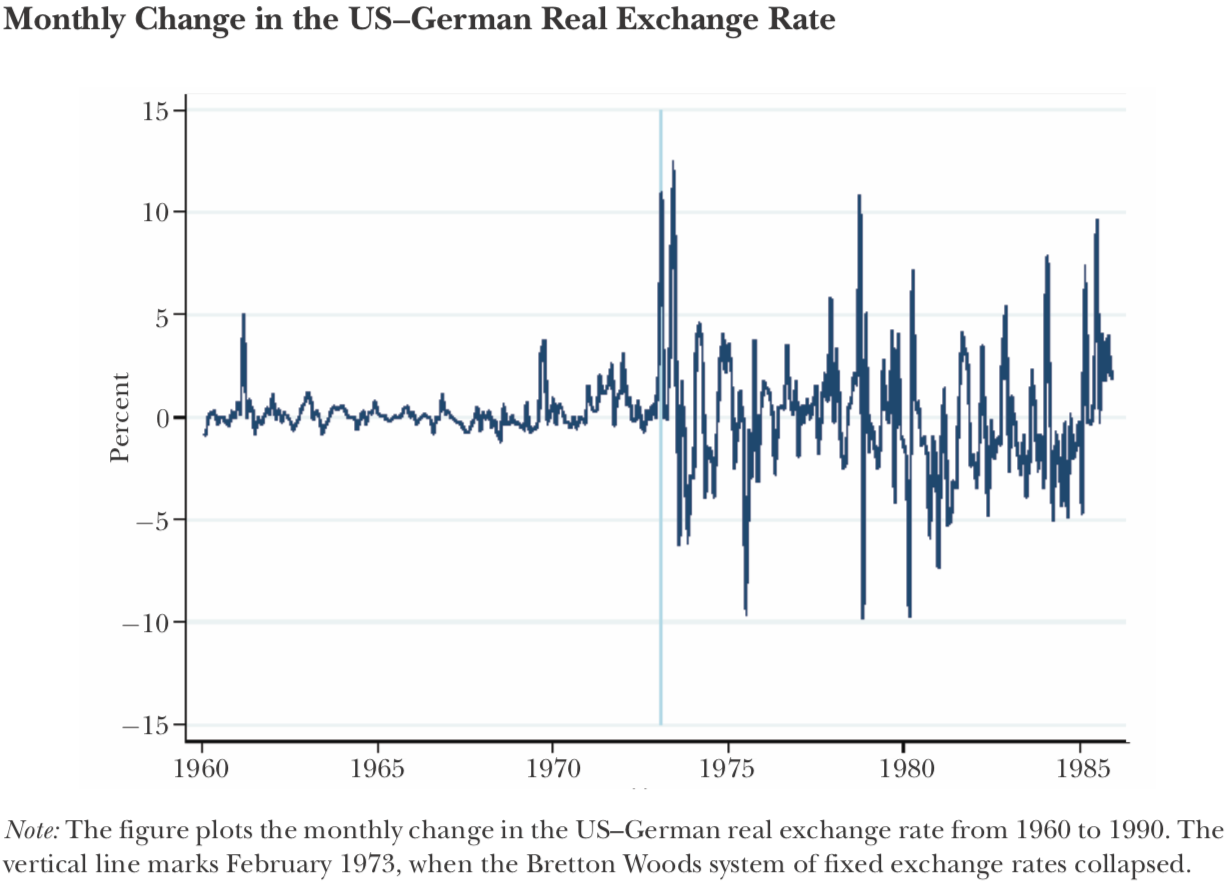
\includegraphics[scale=0.4]{../../Images/NS2018mussa.png}
\end{frame}

\begin{frame}
\frametitle{Discontinuity in High-Frequency}
\begin{itemize}
	\item Nakamura and Steinsson (2018) look at response of bond yields within minutes of FOMC announcements.
	\begin{itemize}
		\item Identifying assumption: Responses to unexpected Fed policies dominate changes in bond yields in these narrow windows.
%		\item Compare nominal Treasuries to TIPS (inflation-indexed) to back out effect on real interest rate vs. inflation expectations.
	\end{itemize}
%	\item Nakamura and Steinsson (2018) findings:
%	\begin{itemize}
%		\item Monetary shocks have large and persistent effects on real interest rates.
%		\item Monetary shocks have small effects on expected inflation at short horizons ($<$ 1 year) and grows to a large effect over 2-3 years (hump shaped response).
%	\end{itemize}
\end{itemize}
\centering
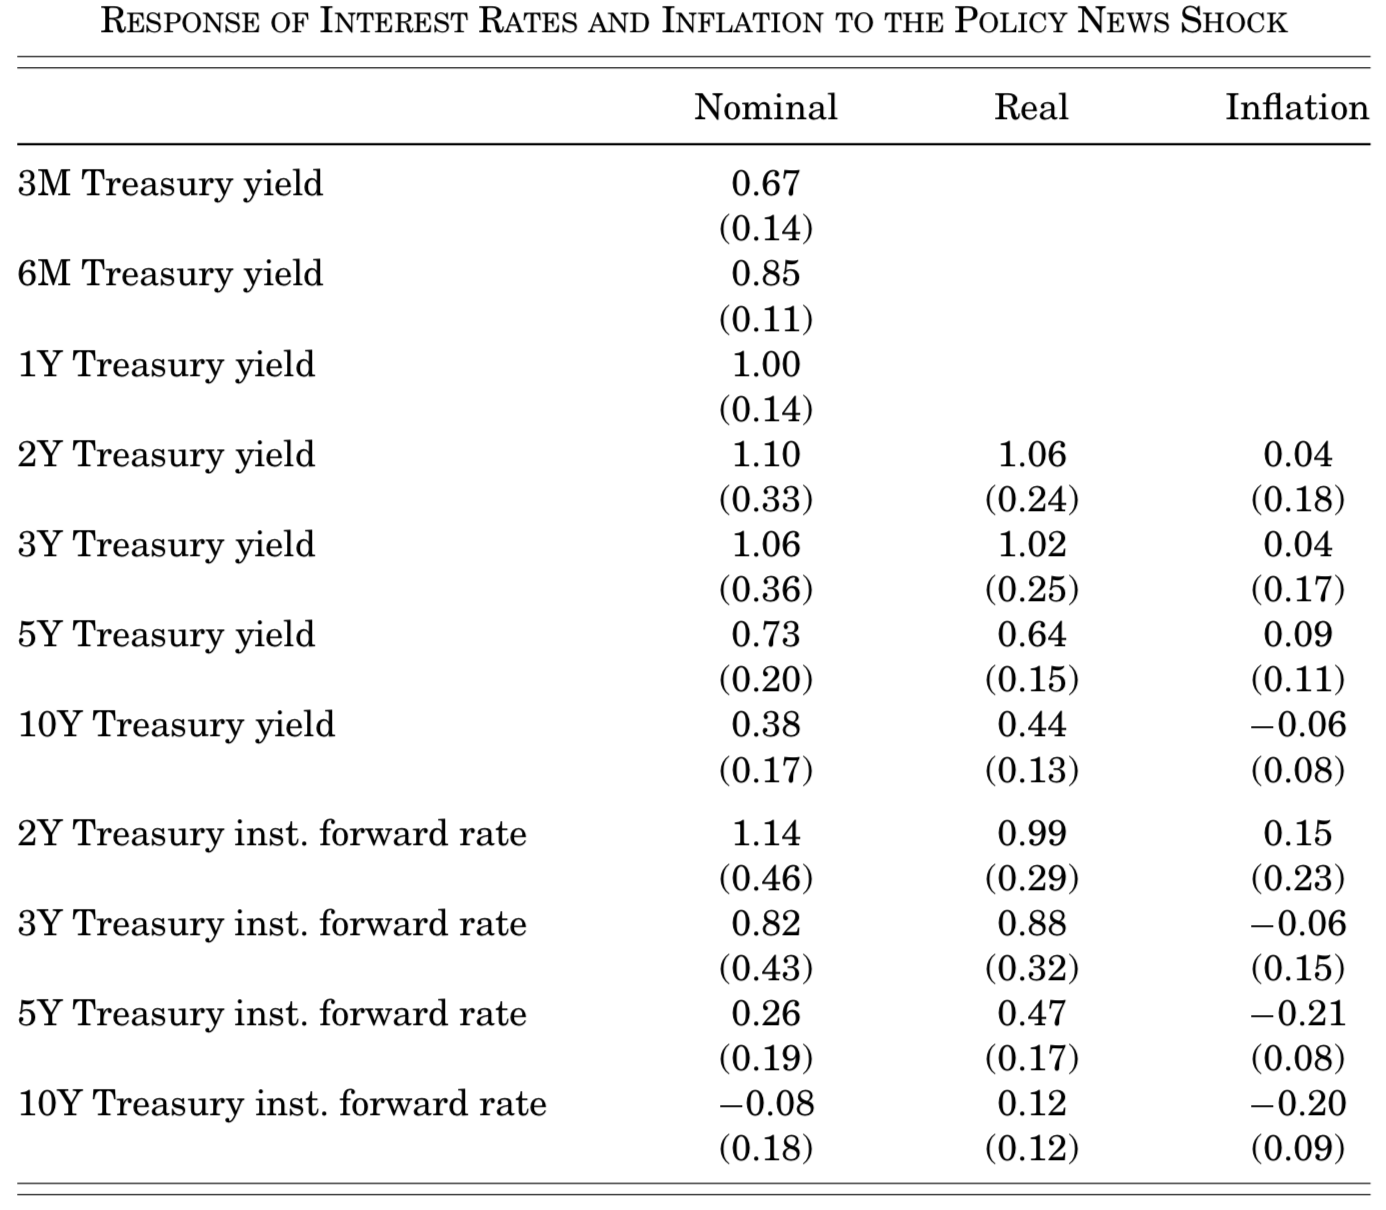
\includegraphics[scale=0.3]{../../Images/NS2018realrate.png}
\end{frame}

%%%%%%%%%%%%%%%%%%%%%%%%%%%%%%%%%%%%%%%%%%%%%%%%%%
\subsection{Narrative}
%%%%%%%%%%%%%%%%%%%%%%%%%%%%%%%%%%%%%%%%%%%%%%%%%%

\begin{frame}
\frametitle{Narrative Approach}
\begin{itemize}
	\item Narrative approach of Romer and Romer (1989)
	\begin{itemize}
		\item Identify exogenous monetary shocks by using historical record to argue what changes in policy were unexpected.
	\end{itemize}
\end{itemize}
\centering
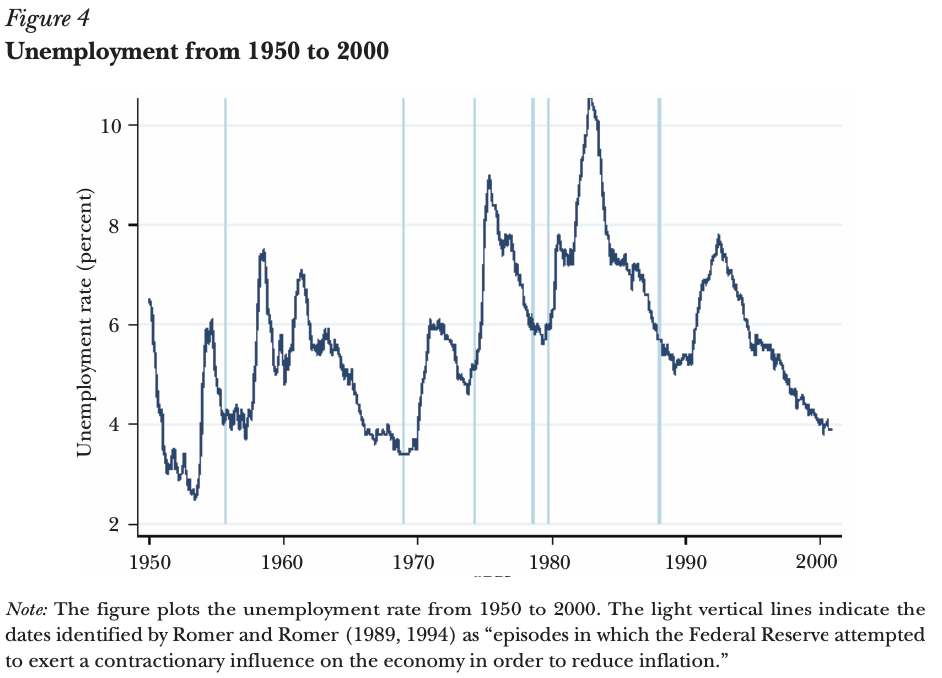
\includegraphics[scale=0.55]{../../Images/NS2018narrative.png}
\end{frame}

\begin{frame}
\frametitle{Narrative Approach}
\begin{itemize}
	\item Narrative approach of Romer and Romer (1989)
	\begin{itemize}
		\item Look at impulse responses only to exogenous shocks.
	\end{itemize}
\begin{center}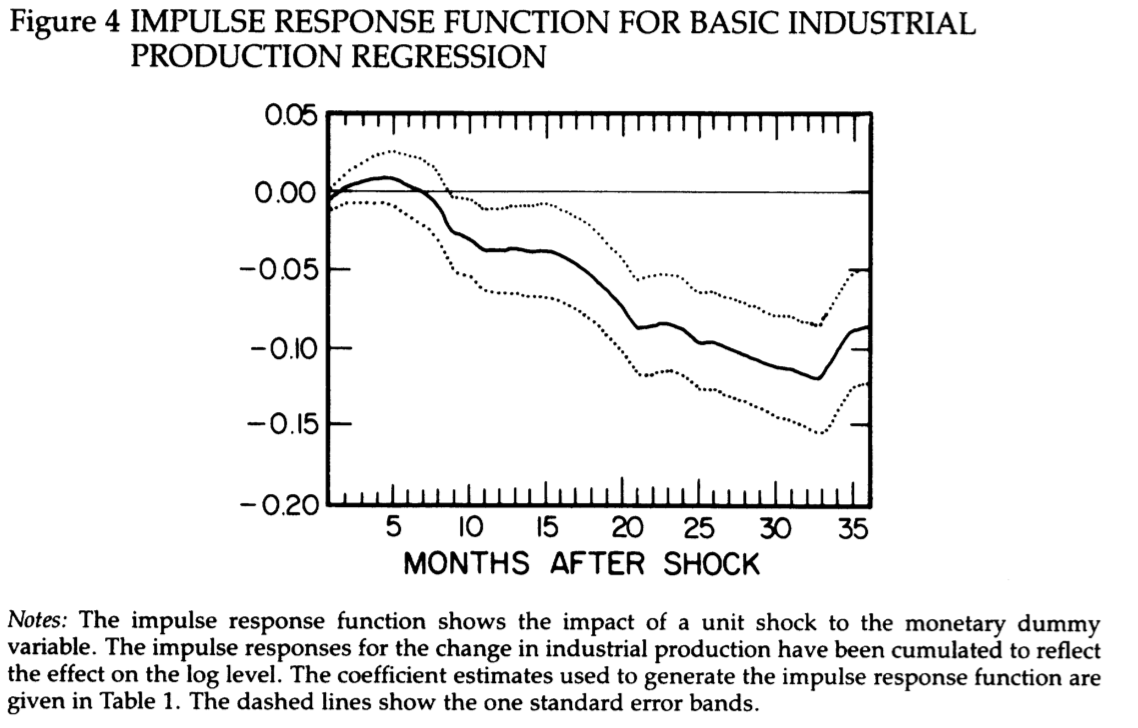
\includegraphics[scale=0.4]{../../Images/RR1989IP.png}\end{center}
	\item Exogeneity assumptions questioned by Shapiro (1994) and Leeper (1997).
\end{itemize}
\end{frame}

%%%%%%%%%%%%%%%%%%%%%%%%%%%%%%%%%%%%%%%%%%%%%%%%%%
\subsection{Controlling for Confounders}
%%%%%%%%%%%%%%%%%%%%%%%%%%%%%%%%%%%%%%%%%%%%%%%%%%

\begin{frame}
\frametitle{Controlling for Confounders}
\begin{itemize}
	\item Endogenous monetary policy is based on the central banks assessment of where the economy is heading.
	\begin{itemize}
		\item[$\Rightarrow$] To account for endogenous policy, need to know the information available to the central bank.
	\end{itemize}
	\item Romer and Romer (2004) use the Federal Reserve Boards internal forecasts (``Greenbook'') to control for the endogenous component of monetary policy:
	\begin{align*}
		\Delta ff_m&=\alpha+\beta ffb_m + \sum_{i=-1}^2 \gamma_i\tilde{\Delta y}_{mi}+ \sum_{i=-1}^2 \lambda_i(\tilde{\Delta y}_{mi}-\tilde{\Delta y}_{m-1,i}) \\
		&+ \sum_{i=-1}^2 \varphi_i\tilde{\pi}_{mi}+ \sum_{i=-1}^2 \theta_i(\tilde{\pi}_{mi}-\tilde{\pi}_{m-1,i})+\rho\tilde{u}_{m0}+\epsilon_m
	\end{align*}
	\item Residuals $\epsilon_m$ are the monetary policy shocks.
\end{itemize}
\end{frame}


\begin{frame}
\frametitle{Controlling for Confounders}
\begin{itemize}
	\item Construct IRF for industrial production based on $\epsilon_m$: \\
\end{itemize}
\centering
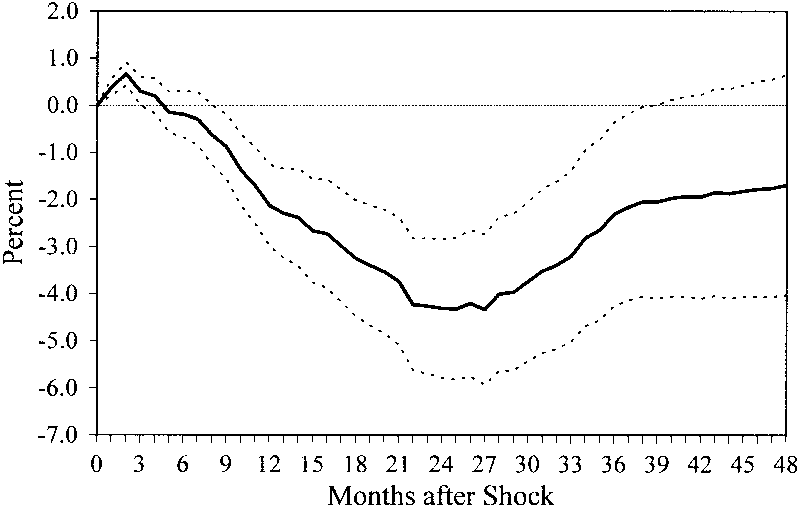
\includegraphics[scale=0.4]{../../Images/RR2004irfy.png}
\end{frame}



\begin{frame}
\frametitle{Summary: Strong Evidence of Non-Neutrality}
\begin{itemize}
	\item We examined evidence from a wide variety of sources and methods:
	\begin{itemize}
		\item Large shocks.
		\item Discontinuity-based approach.
		\item Narrative approach.
		\item Controlling for confounders (inc. VAR).
	\end{itemize}
	\item Strong evidence that money is non-neutral: it has effects on real economy.
\end{itemize}
\end{frame}

\section{Next Steps}

\begin{frame}
\frametitle{Next Steps}
\begin{itemize}
	\item Need to move beyond Classical Dichotomy.
	\item Build simplest(?) model in which money is neutral in the long-run but not in the short-run.
\end{itemize}
\end{frame}


\end{document}